% Options for packages loaded elsewhere
\PassOptionsToPackage{unicode}{hyperref}
\PassOptionsToPackage{hyphens}{url}
%
\documentclass[
  ignorenonframetext,
]{beamer}
\usepackage{pgfpages}
\setbeamertemplate{caption}[numbered]
\setbeamertemplate{caption label separator}{: }
\setbeamercolor{caption name}{fg=normal text.fg}
\beamertemplatenavigationsymbolsempty
% Prevent slide breaks in the middle of a paragraph
\widowpenalties 1 10000
\raggedbottom
\setbeamertemplate{part page}{
  \centering
  \begin{beamercolorbox}[sep=16pt,center]{part title}
    \usebeamerfont{part title}\insertpart\par
  \end{beamercolorbox}
}
\setbeamertemplate{section page}{
  \centering
  \begin{beamercolorbox}[sep=12pt,center]{part title}
    \usebeamerfont{section title}\insertsection\par
  \end{beamercolorbox}
}
\setbeamertemplate{subsection page}{
  \centering
  \begin{beamercolorbox}[sep=8pt,center]{part title}
    \usebeamerfont{subsection title}\insertsubsection\par
  \end{beamercolorbox}
}
\AtBeginPart{
  \frame{\partpage}
}
\AtBeginSection{
  \ifbibliography
  \else
    \frame{\sectionpage}
  \fi
}
\AtBeginSubsection{
  \frame{\subsectionpage}
}
\usepackage{lmodern}
\usepackage{amssymb,amsmath}
\usepackage{ifxetex,ifluatex}
\ifnum 0\ifxetex 1\fi\ifluatex 1\fi=0 % if pdftex
  \usepackage[T1]{fontenc}
  \usepackage[utf8]{inputenc}
  \usepackage{textcomp} % provide euro and other symbols
\else % if luatex or xetex
  \usepackage{unicode-math}
  \defaultfontfeatures{Scale=MatchLowercase}
  \defaultfontfeatures[\rmfamily]{Ligatures=TeX,Scale=1}
\fi
% Use upquote if available, for straight quotes in verbatim environments
\IfFileExists{upquote.sty}{\usepackage{upquote}}{}
\IfFileExists{microtype.sty}{% use microtype if available
  \usepackage[]{microtype}
  \UseMicrotypeSet[protrusion]{basicmath} % disable protrusion for tt fonts
}{}
\makeatletter
\@ifundefined{KOMAClassName}{% if non-KOMA class
  \IfFileExists{parskip.sty}{%
    \usepackage{parskip}
  }{% else
    \setlength{\parindent}{0pt}
    \setlength{\parskip}{6pt plus 2pt minus 1pt}}
}{% if KOMA class
  \KOMAoptions{parskip=half}}
\makeatother
\usepackage{xcolor}
\IfFileExists{xurl.sty}{\usepackage{xurl}}{} % add URL line breaks if available
\IfFileExists{bookmark.sty}{\usepackage{bookmark}}{\usepackage{hyperref}}
\hypersetup{
  pdftitle={MA8701 Advanced methods in statistical inference and learning},
  pdfauthor={Mette Langaas IMF/NTNU},
  hidelinks,
  pdfcreator={LaTeX via pandoc}}
\urlstyle{same} % disable monospaced font for URLs
\newif\ifbibliography
\usepackage{color}
\usepackage{fancyvrb}
\newcommand{\VerbBar}{|}
\newcommand{\VERB}{\Verb[commandchars=\\\{\}]}
\DefineVerbatimEnvironment{Highlighting}{Verbatim}{commandchars=\\\{\}}
% Add ',fontsize=\small' for more characters per line
\usepackage{framed}
\definecolor{shadecolor}{RGB}{248,248,248}
\newenvironment{Shaded}{\begin{snugshade}}{\end{snugshade}}
\newcommand{\AlertTok}[1]{\textcolor[rgb]{0.94,0.16,0.16}{#1}}
\newcommand{\AnnotationTok}[1]{\textcolor[rgb]{0.56,0.35,0.01}{\textbf{\textit{#1}}}}
\newcommand{\AttributeTok}[1]{\textcolor[rgb]{0.77,0.63,0.00}{#1}}
\newcommand{\BaseNTok}[1]{\textcolor[rgb]{0.00,0.00,0.81}{#1}}
\newcommand{\BuiltInTok}[1]{#1}
\newcommand{\CharTok}[1]{\textcolor[rgb]{0.31,0.60,0.02}{#1}}
\newcommand{\CommentTok}[1]{\textcolor[rgb]{0.56,0.35,0.01}{\textit{#1}}}
\newcommand{\CommentVarTok}[1]{\textcolor[rgb]{0.56,0.35,0.01}{\textbf{\textit{#1}}}}
\newcommand{\ConstantTok}[1]{\textcolor[rgb]{0.00,0.00,0.00}{#1}}
\newcommand{\ControlFlowTok}[1]{\textcolor[rgb]{0.13,0.29,0.53}{\textbf{#1}}}
\newcommand{\DataTypeTok}[1]{\textcolor[rgb]{0.13,0.29,0.53}{#1}}
\newcommand{\DecValTok}[1]{\textcolor[rgb]{0.00,0.00,0.81}{#1}}
\newcommand{\DocumentationTok}[1]{\textcolor[rgb]{0.56,0.35,0.01}{\textbf{\textit{#1}}}}
\newcommand{\ErrorTok}[1]{\textcolor[rgb]{0.64,0.00,0.00}{\textbf{#1}}}
\newcommand{\ExtensionTok}[1]{#1}
\newcommand{\FloatTok}[1]{\textcolor[rgb]{0.00,0.00,0.81}{#1}}
\newcommand{\FunctionTok}[1]{\textcolor[rgb]{0.00,0.00,0.00}{#1}}
\newcommand{\ImportTok}[1]{#1}
\newcommand{\InformationTok}[1]{\textcolor[rgb]{0.56,0.35,0.01}{\textbf{\textit{#1}}}}
\newcommand{\KeywordTok}[1]{\textcolor[rgb]{0.13,0.29,0.53}{\textbf{#1}}}
\newcommand{\NormalTok}[1]{#1}
\newcommand{\OperatorTok}[1]{\textcolor[rgb]{0.81,0.36,0.00}{\textbf{#1}}}
\newcommand{\OtherTok}[1]{\textcolor[rgb]{0.56,0.35,0.01}{#1}}
\newcommand{\PreprocessorTok}[1]{\textcolor[rgb]{0.56,0.35,0.01}{\textit{#1}}}
\newcommand{\RegionMarkerTok}[1]{#1}
\newcommand{\SpecialCharTok}[1]{\textcolor[rgb]{0.00,0.00,0.00}{#1}}
\newcommand{\SpecialStringTok}[1]{\textcolor[rgb]{0.31,0.60,0.02}{#1}}
\newcommand{\StringTok}[1]{\textcolor[rgb]{0.31,0.60,0.02}{#1}}
\newcommand{\VariableTok}[1]{\textcolor[rgb]{0.00,0.00,0.00}{#1}}
\newcommand{\VerbatimStringTok}[1]{\textcolor[rgb]{0.31,0.60,0.02}{#1}}
\newcommand{\WarningTok}[1]{\textcolor[rgb]{0.56,0.35,0.01}{\textbf{\textit{#1}}}}
\usepackage{longtable,booktabs}
\usepackage{caption}
% Make caption package work with longtable
\makeatletter
\def\fnum@table{\tablename~\thetable}
\makeatother
\usepackage{graphicx,grffile}
\makeatletter
\def\maxwidth{\ifdim\Gin@nat@width>\linewidth\linewidth\else\Gin@nat@width\fi}
\def\maxheight{\ifdim\Gin@nat@height>\textheight\textheight\else\Gin@nat@height\fi}
\makeatother
% Scale images if necessary, so that they will not overflow the page
% margins by default, and it is still possible to overwrite the defaults
% using explicit options in \includegraphics[width, height, ...]{}
\setkeys{Gin}{width=\maxwidth,height=\maxheight,keepaspectratio}
% Set default figure placement to htbp
\makeatletter
\def\fps@figure{htbp}
\makeatother
\setlength{\emergencystretch}{3em} % prevent overfull lines
\providecommand{\tightlist}{%
  \setlength{\itemsep}{0pt}\setlength{\parskip}{0pt}}
\setcounter{secnumdepth}{-\maxdimen} % remove section numbering

\title{MA8701 Advanced methods in statistical inference and learning}
\subtitle{L3: Shrinkage - algorithm, variants, GLM}
\author{Mette Langaas IMF/NTNU}
\date{23 January, 2021}

\begin{document}
\frame{\titlepage}

\begin{frame}{Shrinkage - second act}
\protect\hypertarget{shrinkage---second-act}{}

\begin{block}{Literature L3}

\begin{itemize}
\item
  {[}ELS{]} The Elements of Statistical Learning: Data Mining,
  Inference, and Prediction, Second Edition (Springer Series in
  Statistics, 2009) by Trevor Hastie, Robert Tibshirani, and Jerome
  Friedman.
  \href{https://web.stanford.edu/~hastie/Papers/ESLII.pdf}{Ebook}.
  Chapter 4.4.1-4.4.3 (4.4.4 is covered in 3.2 of HTW).
\item
  {[}HTW{]} Hastie, Tibshirani, Wainwrigh: ``Statistical Learning with
  Sparsity: The Lasso and Generalizations''. CRC press.
  \href{https://trevorhastie.github.io/}{Ebook}. Chapter 2.4
  (understanding from 5.4 will be presented - but not on reading list),
  3.1-3.2,3.7 4.1-4.3,4.5-4.6 (but only from a practical view for ch 4)
\end{itemize}

\end{block}

\end{frame}

\begin{frame}{Lasso}
\protect\hypertarget{lasso}{}

What do we know from L2?

We forgot to say that

\begin{itemize}
\tightlist
\item
  the acronym is \emph{Least Absolute Shrinkage and Selection Operator},
  and that the
\item
  lasso was invented by Robert Tibshirani and published in an article in
  \href{https://www.jstor.org/stable/2346178?seq=1}{JRSSB in 1996}
\end{itemize}

We still work on the linear regression case - with continuous response.

\end{frame}

\begin{frame}

\begin{block}{Computations of the lasso solutions}

(HTW 2.4)

\begin{itemize}
\tightlist
\item
  Focus is on the Coordinate descent algorithm, where
\item
  soft thresholding plays an important role.
\item
  Also mention the concept of subgradients (from HTW 5.4 - not on the
  reading list).
\end{itemize}

See \href{slides\%20link}{slides from guest lecturer Benjamin Dunn}

\end{block}

\end{frame}

\begin{frame}

\textbf{Group discussion:}

Write down in pseudo code the steps of the cyclic coordinate descent
algorithm.

\end{frame}

\begin{frame}

\end{frame}

\begin{frame}

\begin{block}{Coordinate descent}

(Result HTW page 110): Additive function to minimize:
\[ f(\beta)=g(\beta)+\sum_{j=1}^p h_j(\beta_j)\]

\(g\) differentiable and convex, \(h\) univariate and convex. It is
found that the coordinate descent algorithm is \emph{guaranteed to
converge} to the global minimizer.

\end{block}

\end{frame}

\begin{frame}

\begin{block}{Generalizations of the lasso penalty}

(HTW 4.1-4.3, 4.5-4.6: NB only from a practical point of view)

See \href{slides\%20link}{slides from guest lecturer Benjamin Dunn}

The main goal of this part is to

\begin{itemize}
\tightlist
\item
  know about these special versions of the lasso, and
\item
  to see which practical data situation these can be smart to use.
\end{itemize}

Maybe one of these is suitable for Data analysis project 1?

Theoretical properties and algorithmic details are not on the reading
list.

\end{block}

\end{frame}

\begin{frame}

\textbf{Group activity:}

(choose one variant to work with)

For the lasso variants

\begin{itemize}
\tightlist
\item
  the elastic net {[}HTW 4.2{]}
\item
  the group lasso {[}HTW 4.3{]}
\item
  the fused lasso {[}HTW 4.5{]} 
\end{itemize}

write down

\begin{itemize}
\tightlist
\item
  which variation on the classic lasso penalty is used (write down the
  penalty part of the minimization problem)
\item
  make a drawing of the penalty (comparable to the sphere for ridge and
  the diamond for lasso)
\item
  in which practical data analysis situation is this variation used
  (e.g.~when many correlated variables are present, when the covariates
  have a natural group structure, \ldots)
\item
  anything else you found interesting?
\end{itemize}

\end{frame}

\begin{frame}

\end{frame}

\begin{frame}{Generalized linear models}
\protect\hypertarget{generalized-linear-models}{}

(HTW 3.1, 3.2, and TMA4315 GLM background)

\begin{block}{The model}

The GLM model has three ingredients:

\begin{enumerate}
[1)]
\tightlist
\item
  Random component
\item
  Systematic component
\item
  Link function
\end{enumerate}

We look into that for the normal and binomial distribution - to get
multiple linear regression and logistic regression.

\begin{itemize}
\tightlist
\item
  \href{classnotelink}{Write in class}
\item
  Poll on standardization and centering.
\end{itemize}

\end{block}

\end{frame}

\begin{frame}

\end{frame}

\begin{frame}

\begin{block}{Explaining \(\beta\) in logistic regression}

\begin{itemize}
\item
  The ratio \(\frac{P(Y_i=1)}{P(Y_i=0)}=\frac{\pi_i}{1-\pi_1}\) is
  called the \emph{odds}.
\item
  If \(\pi_i=\frac{1}{2}\) then the odds is \(1\), and if
  \(\pi_i=\frac{1}{4}\) then the odds is \(\frac{1}{3}\). We may make a
  table for probability vs.~odds in R:
\end{itemize}

\begin{table}[H]
\centering
\begin{tabular}{l|r|r|r|r|r|r|r|r|r}
\hline
pivec & 0.10 & 0.20 & 0.30 & 0.40 & 0.5 & 0.6 & 0.70 & 0.8 & 0.9\\
\hline
odds & 0.11 & 0.25 & 0.43 & 0.67 & 1.0 & 1.5 & 2.33 & 4.0 & 9.0\\
\hline
\end{tabular}
\end{table}

\begin{itemize}
\tightlist
\item
  Odds may be seen to be a better scale than probability to represent
  chance, and is used in betting. In addition, odds are unbounded above.
\end{itemize}

\end{block}

\end{frame}

\begin{frame}

We look at the link function (inverse of the response function). Let us
assume that our linear predictor has \(k\) covariates present

\begin{align*}
\eta_i&= \beta_0+\beta_1 x_{i1}+\beta_2 x_{i2}+\cdots + \beta_k x_{ik}\\
\pi_i&= \frac{\exp(\eta_i)}{1+\exp(\eta_i)}\\
\eta_i&=\ln(\frac{\pi_i}{1-\pi_i})\\
\ln(\frac{\pi_i}{1-\pi_i})&=\beta_0+\beta_1 x_{i1}+\beta_2 x_{i2}+\cdots + \beta_k x_{ik}\\
\frac{\pi_i}{1-\pi_i}=&\frac{P(Y_i=1)}{P(Y_i=0)}=\exp(\beta_0)\cdot \exp(\beta_1 x_{i1})\cdots\exp(\beta_k x_{ik})
\end{align*}

We have a \emph{multiplicative model} for the odds.

\end{frame}

\begin{frame}

\textbf{So, what if we increase \(x_{1i}\) to \(x_{1i}+1\)?}

If the covariate \(x_{1i}\) increases by one unit (while all other
covariates are kept fixed) then the odds is multiplied by
\(\exp(\beta_1)\):

\begin{align*}
\frac{P(Y_i=1\mid x_{i1}+1)}{P(Y_i=0)\mid x_{i1}+1)}&=\exp(\beta_0)\cdot \exp(\beta_1 (x_{i1}+1))\cdots\exp(\beta_k x_{ik})\\
&=\exp(\beta_0)\cdot \exp(\beta_1 x_{i1})\exp(\beta_1)\cdots\exp(\beta_k x_{ik})\\
&=\frac{P(Y_i=1\mid x_{i1})}{P(Y_i=0\mid x_{i1})}\cdot \exp(\beta_1)\\
\end{align*}

This means that if \(x_{i1}\) increases by \(1\) then: if \(\beta_1<0\)
we get a decrease in the odds, if \(\beta_1=0\) no change, and if
\(\beta_1>0\) we have an increase. In the logit model \(\exp(\beta_1)\)
is easier to interpret than \(\beta_1\).

\end{frame}

\begin{frame}

The response function as a function of the covariate \(x\) and not of
\(\eta\). Solid lines: \(\beta_0=0\) and \(\beta_1\) is \(0.8\) (blue),
\(1\) (red) and \(2\) (orange), and dashed lines with \(\beta_0=1\).

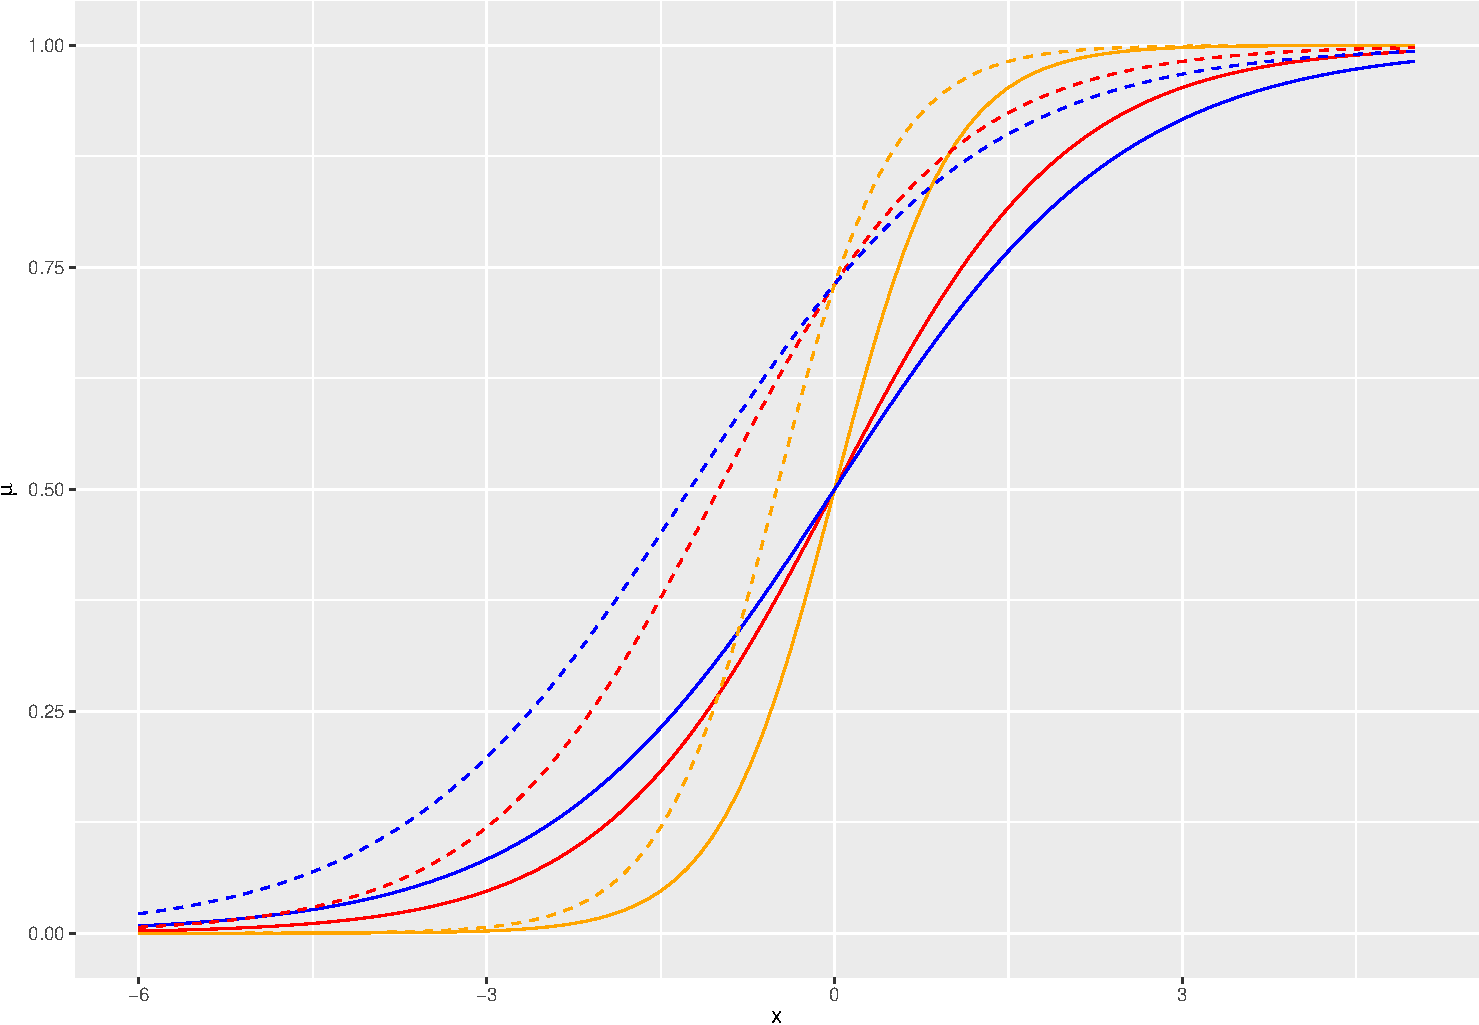
\includegraphics{L3_files/figure-beamer/unnamed-chunk-2-1.pdf}

\end{frame}

\begin{frame}

\begin{block}{Parameter estimation}

\begin{itemize}
\item
  Maximum likelihood estimation = maximize the likelihood of the data
  \(\cal L(\beta_0,\beta; {\bf y}, {\bf X})\).
\item
  For penalized method we instead minimize the negative loglikelihood
  scaled with \(\frac{1}{N}\).
\item
  The ridge and lasso penalty is added to the scaled negative
  loglikelihood.
\item
  We write this out for the normal and binomial distribution.
\item
  \href{classnotelink}{Write in class}
\end{itemize}

\end{block}

\end{frame}

\begin{frame}

\end{frame}

\begin{frame}

\begin{block}{Algorithms}

\begin{itemize}
\tightlist
\item
  The likelihood for the GLM is differentiable, and the ridge and lasso
  objective functions are convex - and can be solved with socalled
  ``standard convex optimization methods''.
\item
  But, by popular demand also special algorithms are available -
  building on the cyclic coordinate descent.
\end{itemize}

To understand the (ridge and) lasso logistic regression we first look at
the \emph{iteratively reweighted least squares} (IRLS) - as a result of
the Newton Raphson method.

\end{block}

\end{frame}

\begin{frame}

\end{frame}

\begin{frame}[fragile]

\begin{block}{Lasso logistic regression fitting algoritm}

(HTW page 116)

\begin{Shaded}
\begin{Highlighting}[]
\NormalTok{OUTER LOOP}\OperatorTok{:}\StringTok{ }\NormalTok{start with lambdamax and decrement}

\NormalTok{      MIDDLE }\KeywordTok{LOOP}\NormalTok{ (with warm start) }
         
\NormalTok{         compute quadratic approximation }\KeywordTok{Q}\NormalTok{(beta0,beta) }
         \ControlFlowTok{for}\NormalTok{ current beta}\OperatorTok{-}\NormalTok{estimates}
         
         
         
\NormalTok{              INNER LOOP}\OperatorTok{:}\StringTok{ }\NormalTok{cyclic coordinate descent}
\NormalTok{              to minimize Q added the lasso penalty}
\end{Highlighting}
\end{Shaded}

\end{block}

\end{frame}

\begin{frame}

\begin{block}{Criteria for choosing \(\lambda\)}

We use cross-validation to choose \(\lambda\).

For regression we choose \(\lambda\) by minimizing the (mean) squared
error.

For (ridge and) lasso logistic regression we may choose:

\begin{itemize}
\tightlist
\item
  misclassification error rate on the validation set
\item
  ROC-AUC
\item
  binomial deviance
\end{itemize}

\end{block}

\end{frame}

\begin{frame}

\begin{block}{Confusion matrix, sensitivity, specificity}

(from TMA4268)

In a two class problem - assume the classes are labelled ``-'' (non
disease,0) and ``+'' (disease,1). In a population setting we define the
following event and associated number of observations.

\begin{longtable}[]{@{}llll@{}}
\toprule
& Predicted - & Predicted + & Total\tabularnewline
\midrule
\endhead
True - & True Negative TN & False Positive FP & N\tabularnewline
True + & False Negative FN & True Positive TP & P\tabularnewline
Total & N* & P* &\tabularnewline
\bottomrule
\end{longtable}

(N in this context not to be confused with our sample size\ldots)

\end{block}

\end{frame}

\begin{frame}

\textbf{Sensitivity} (recall) is the proportion of correctly classified
positive observations:
\(\frac{\# \text{True Positive}}{\# \text{Condition Positive}}=\frac{\text{TP}}{\text{P}}\).

\textbf{Specificity} is the proportion of correctly classified negative
observations:
\(\frac{\# \text{True Negative}}{\# \text{Condition Negative}}=\frac{\text{TN}}{\text{N}}\).

We would like that a classification rule have both a high sensitivity
and a high specificity.

\end{frame}

\begin{frame}

Other useful quantities:

\begin{longtable}[]{@{}lll@{}}
\toprule
\begin{minipage}[b]{0.36\columnwidth}\raggedright
Name\strut
\end{minipage} & \begin{minipage}[b]{0.20\columnwidth}\raggedright
Definition\strut
\end{minipage} & \begin{minipage}[b]{0.36\columnwidth}\raggedright
Synonoms\strut
\end{minipage}\tabularnewline
\midrule
\endhead
\begin{minipage}[t]{0.36\columnwidth}\raggedright
False positive rate\strut
\end{minipage} & \begin{minipage}[t]{0.20\columnwidth}\raggedright
FP/N\strut
\end{minipage} & \begin{minipage}[t]{0.36\columnwidth}\raggedright
Type I error, 1-specificity\strut
\end{minipage}\tabularnewline
\begin{minipage}[t]{0.36\columnwidth}\raggedright
True positive rate\strut
\end{minipage} & \begin{minipage}[t]{0.20\columnwidth}\raggedright
TP/P\strut
\end{minipage} & \begin{minipage}[t]{0.36\columnwidth}\raggedright
1-Type II error, power, sensitivity, recall\strut
\end{minipage}\tabularnewline
\begin{minipage}[t]{0.36\columnwidth}\raggedright
Positive predictive value (PPV)\strut
\end{minipage} & \begin{minipage}[t]{0.20\columnwidth}\raggedright
TP/P*\strut
\end{minipage} & \begin{minipage}[t]{0.36\columnwidth}\raggedright
Precision, 1-false discovery proportion\strut
\end{minipage}\tabularnewline
\begin{minipage}[t]{0.36\columnwidth}\raggedright
Negative predictive value (NPV)\strut
\end{minipage} & \begin{minipage}[t]{0.20\columnwidth}\raggedright
TN/N*\strut
\end{minipage} & \begin{minipage}[t]{0.36\columnwidth}\raggedright
\strut
\end{minipage}\tabularnewline
\bottomrule
\end{longtable}

Where the PPV can be used together with the sensitivity to make a
precision-recall curve more suitable for low case rates.

\end{frame}

\begin{frame}

\begin{block}{ROC curves}

(also from TMA4268)

The receiver operating characteristics (ROC) curve gives a graphical
display of the sensitivity against specificity, as the threshold value
(cut-off on probability of success or disease) is moved over the range
of all possible values. An ideal classifier will give a ROC curve which
hugs the top left corner, while a straight line represents a classifier
with a random guess of the outcome.

\end{block}

\end{frame}

\begin{frame}

\begin{block}{ROC-AUC}

\begin{itemize}
\tightlist
\item
  The \textbf{ROC-AUC} score is the area under the ROC curve. It ranges
  between the values 0 and 1, where a higher value indicates a better
  classifier. 
\item
  The AUC score is useful for comparing the performance of different
  classifiers, as all possible threshold values are taken into account.
\item
  The ROC-AUC is closely connected to the robust U statistics.
\item
  If the prevalence (case proportion) is very low (0.01ish), the ROC-AUC
  may be misleading, and the PR-AUC is more commonly used.
\end{itemize}

\end{block}

\end{frame}

\begin{frame}

\begin{block}{Deviance}

The \emph{deviance} is based on the likelihood ratio test statistic.

The derivation assumes that data can be grouped into covariate patterns,
with \(G\) groups (else interval solutions are used in practice).

\textbf{Saturated model:} If we were to provide a perfect fit to our
data then we would estimate \(\pi_j\) by the observed frequency for the
group, \(\hat{y}_j=y_j\).

\textbf{Candidate model:} the model with the current choice of
\(\lambda\).

\[D_{\lambda}=2(l(\text{saturated model})-l(\text{candidate model}_{\lambda}))\]
The \textbf{null deviance} is replacing the candidate model with a model
where \(\hat{y}_i=\frac{1}{N}\sum_{i=1}^N y_i\) (the case proportion).

\end{block}

\end{frame}

\begin{frame}{Example: South African heart disease}
\protect\hypertarget{example-south-african-heart-disease}{}

(ELS 4.4.2)

\textbf{Group discussion:} Comment on what is done and the results.
Where are the CIs and \(p\)-values for the ridge and lasso version?

\end{frame}

\begin{frame}[fragile]

\begin{block}{Data set}

The data is presented in ELS Section 4.4.2, and downloaded from
\url{http://statweb.stanford.edu/~tibs/ElemStatLearn.1stEd/} with
information in the file \texttt{SAheat.info} and data in
\texttt{SAheart.data}.

\begin{itemize}
\tightlist
\item
  This is a retrospective sample of males in a heart-disease high-risk
  region in South Africa. *It consists of 462 observations on the 10
  variables. All subjects are male in the age range 15-64.
\item
  There are 160 cases (individuals who have suffered from a conorary
  heart disease) and 302 controls (individuals who have not suffered
  from a conorary heart disease).\\
\item
  The overall prevalence in the region was 5.1\%.
\end{itemize}

The response value (\texttt{chd}) and covariates

\begin{itemize}
\tightlist
\item
  \texttt{chd} : conorary heart disease \{yes, no\} coded by the numbers
  \{1, 0\}
\item
  \texttt{sbp} : systolic blood pressure\\
\item
  \texttt{tobacco} : cumulative tobacco (kg)\\
\item
  \texttt{ldl} : low density lipoprotein cholesterol
\item
  \texttt{adiposity} : a numeric vector
\item
  \texttt{famhist} : family history of heart disease. Categorical
  variable with two levels: \{Absent, Present\}.
\item
  \texttt{typea} : type-A behavior
\item
  \texttt{obesity} : a numerical value
\item
  \texttt{alcohol} : current alcohol consumption
\item
  \texttt{age} : age at onset
\end{itemize}

\emph{The goal is to identify important risk factors.}

\end{block}

\end{frame}

\begin{frame}[fragile]

\begin{block}{Data description}

We start by loading and looking at the data:

\begin{Shaded}
\begin{Highlighting}[]
\NormalTok{ds=}\KeywordTok{read.csv}\NormalTok{(}\StringTok{"./SAheart.data"}\NormalTok{,}\DataTypeTok{sep=}\StringTok{","}\NormalTok{)[,}\OperatorTok{-}\DecValTok{1}\NormalTok{]}
\NormalTok{ds}\OperatorTok{$}\NormalTok{chd=}\KeywordTok{as.factor}\NormalTok{(ds}\OperatorTok{$}\NormalTok{chd)}
\NormalTok{ds}\OperatorTok{$}\NormalTok{famhist=}\KeywordTok{as.factor}\NormalTok{(ds}\OperatorTok{$}\NormalTok{famhist)}
\KeywordTok{dim}\NormalTok{(ds)}
\end{Highlighting}
\end{Shaded}

\begin{verbatim}
## [1] 462  10
\end{verbatim}

\begin{Shaded}
\begin{Highlighting}[]
\KeywordTok{colnames}\NormalTok{(ds)}
\end{Highlighting}
\end{Shaded}

\begin{verbatim}
##  [1] "sbp"       "tobacco"   "ldl"       "adiposity" "famhist"   "typea"    
##  [7] "obesity"   "alcohol"   "age"       "chd"
\end{verbatim}

\begin{Shaded}
\begin{Highlighting}[]
\KeywordTok{head}\NormalTok{(ds)}
\end{Highlighting}
\end{Shaded}

\begin{verbatim}
##   sbp tobacco  ldl adiposity famhist typea obesity alcohol age chd
## 1 160   12.00 5.73     23.11 Present    49   25.30   97.20  52   1
## 2 144    0.01 4.41     28.61  Absent    55   28.87    2.06  63   1
## 3 118    0.08 3.48     32.28 Present    52   29.14    3.81  46   0
## 4 170    7.50 6.41     38.03 Present    51   31.99   24.26  58   1
## 5 134   13.60 3.50     27.78 Present    60   25.99   57.34  49   1
## 6 132    6.20 6.47     36.21 Present    62   30.77   14.14  45   0
\end{verbatim}

\begin{Shaded}
\begin{Highlighting}[]
\CommentTok{# to be easier to compare with lasso and ridge, we standardize the xs}
\NormalTok{xs=}\KeywordTok{model.matrix}\NormalTok{(chd}\OperatorTok{~}\NormalTok{.,}\DataTypeTok{data=}\NormalTok{ds)[,}\OperatorTok{-}\DecValTok{1}\NormalTok{] }\CommentTok{# to take care of categorical variables, but not include the intercept column}
\NormalTok{xss=}\KeywordTok{scale}\NormalTok{(xs)}
\NormalTok{ys=}\KeywordTok{as.numeric}\NormalTok{(ds[,}\DecValTok{10}\NormalTok{])}\OperatorTok{-}\DecValTok{1} \CommentTok{# not factor, must be numeric else errors...}
\KeywordTok{head}\NormalTok{(xss)}
\end{Highlighting}
\end{Shaded}

\begin{verbatim}
##          sbp    tobacco        ldl  adiposity famhistPresent      typea
## 1  1.0574173  1.8210988  0.4778941 -0.2951832      1.1845700 -0.4180170
## 2  0.2767892 -0.7893817 -0.1595071  0.4116942     -0.8423609  0.1931344
## 3 -0.9917313 -0.7741412 -0.6085852  0.8833742      1.1845700 -0.1124413
## 4  1.5453098  0.8413521  0.8062523  1.6223824      1.1845700 -0.2142999
## 5 -0.2111033  2.1694532 -0.5989276  0.3050200      1.1845700  0.7024273
## 6 -0.3086818  0.5583142  0.8352251  1.3884702      1.1845700  0.9061444
##       obesity    alcohol       age
## 1 -0.17659445  3.2741887 0.6286543
## 2  0.67064592 -0.6120811 1.3816170
## 3  0.73472292 -0.5405973 0.2179473
## 4  1.41109128  0.2947424 1.0393612
## 5 -0.01284211  1.6459912 0.4233008
## 6  1.12155816 -0.1186384 0.1494961
\end{verbatim}

\begin{Shaded}
\begin{Highlighting}[]
\KeywordTok{table}\NormalTok{(ys)}
\end{Highlighting}
\end{Shaded}

\begin{verbatim}
## ys
##   0   1 
## 302 160
\end{verbatim}

\begin{Shaded}
\begin{Highlighting}[]
\NormalTok{dss=}\KeywordTok{data.frame}\NormalTok{(ys,xss)}
\KeywordTok{colnames}\NormalTok{(dss)[}\DecValTok{1}\NormalTok{]=}\StringTok{"chd"}
\end{Highlighting}
\end{Shaded}

The coloring is done according to the response variable, where green
represents a case \(Y=1\) and red represents a control \(Y=0\).

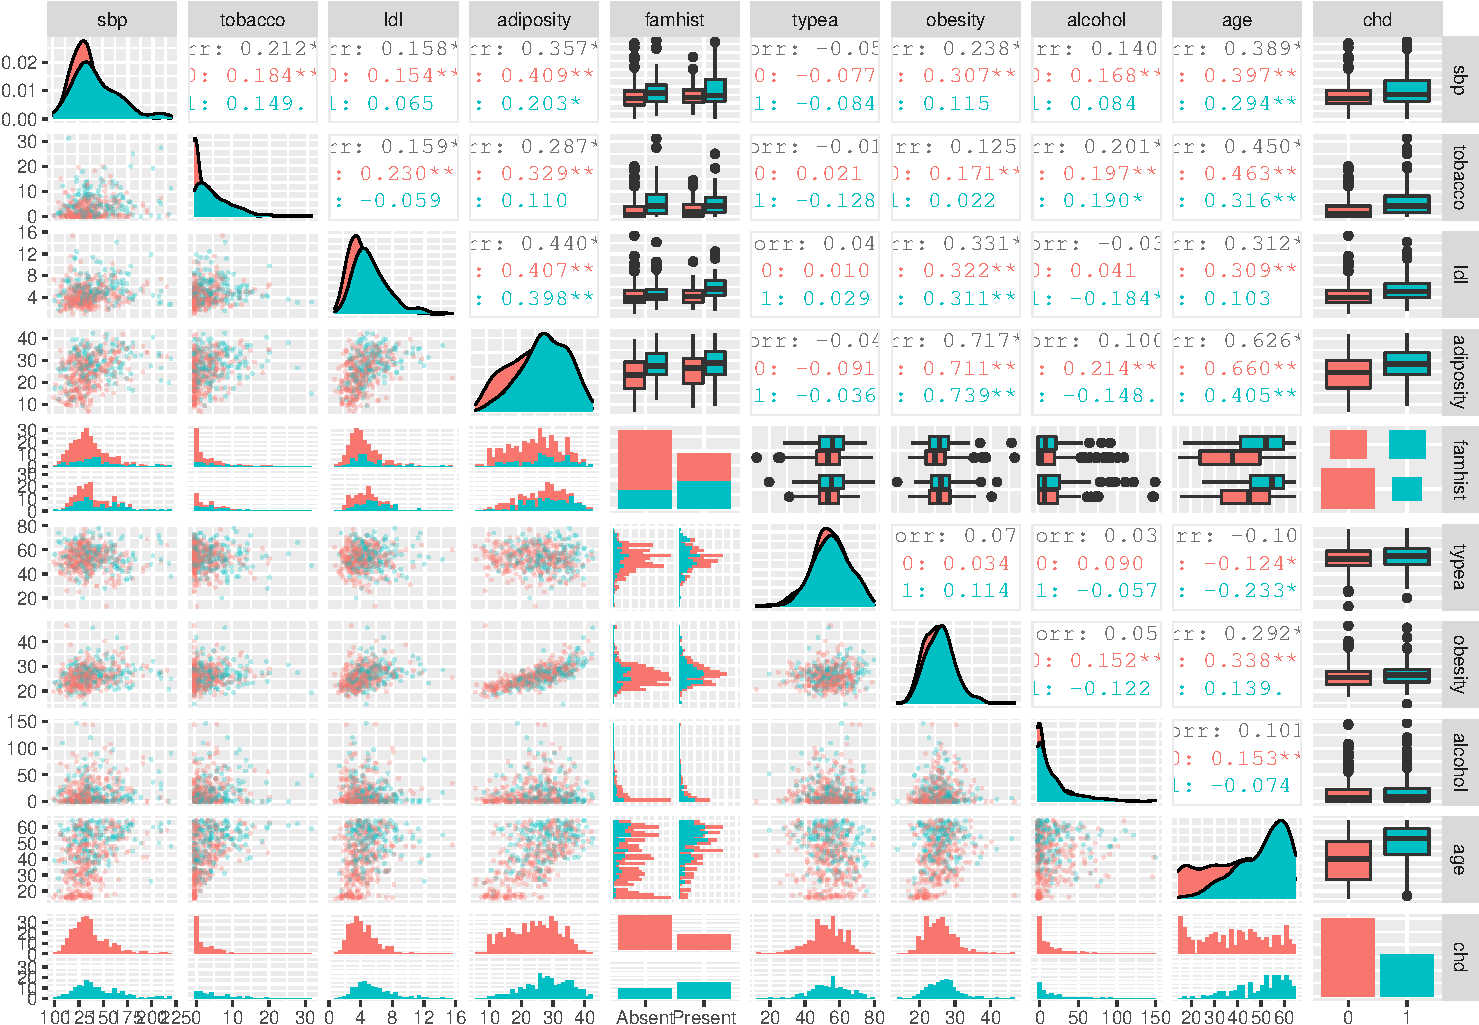
\includegraphics{L3_files/figure-beamer/unnamed-chunk-5-1.pdf}
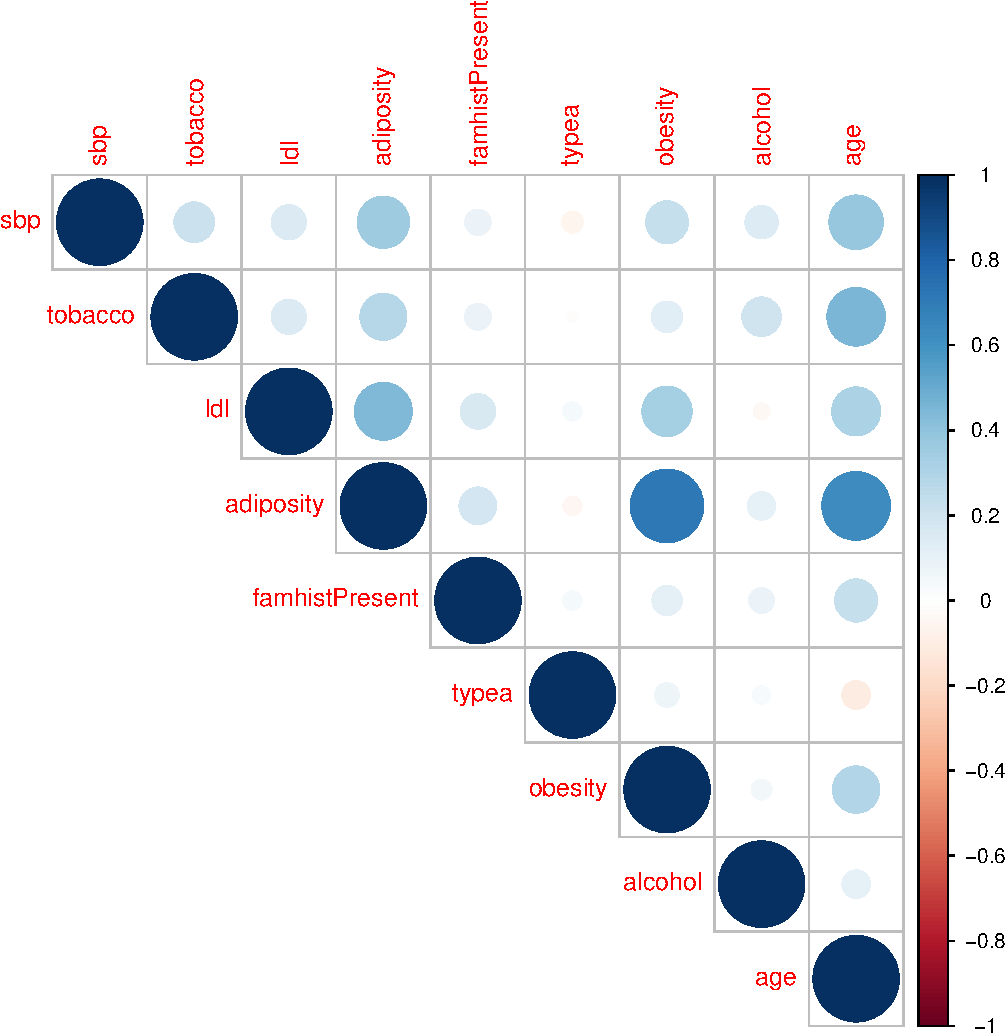
\includegraphics{L3_files/figure-beamer/unnamed-chunk-5-2.pdf}
\textbf{Q:} Comment on the correlation between covariates, and what that
may lead to?

\end{block}

\end{frame}

\begin{frame}[fragile]

\begin{block}{Logistic regression}

We now fit a (multiple) logistic regression model using the \texttt{glm}
function and the full data set. In order to fit a logistic model, the
\texttt{family} argument must be set equal to \texttt{="binomial"}. The
\texttt{summary} function prints out the estimates of the coefficients,
their standard errors and z-values. As for a linear regression model,
the significant coefficients are indicated by stars where the
significant codes are included in the \texttt{R} printout.

\begin{Shaded}
\begin{Highlighting}[]
\NormalTok{glm_heart =}\StringTok{ }\KeywordTok{glm}\NormalTok{(chd}\OperatorTok{~}\NormalTok{.,}\DataTypeTok{data=}\NormalTok{dss, }\DataTypeTok{family=}\StringTok{"binomial"}\NormalTok{)}
\KeywordTok{summary}\NormalTok{(glm_heart)}
\end{Highlighting}
\end{Shaded}

\begin{verbatim}
## 
## Call:
## glm(formula = chd ~ ., family = "binomial", data = dss)
## 
## Deviance Residuals: 
##     Min       1Q   Median       3Q      Max  
## -1.7781  -0.8213  -0.4387   0.8889   2.5435  
## 
## Coefficients:
##                 Estimate Std. Error z value Pr(>|z|)    
## (Intercept)    -0.878545   0.123218  -7.130  1.0e-12 ***
## sbp             0.133308   0.117452   1.135 0.256374    
## tobacco         0.364578   0.122187   2.984 0.002847 ** 
## ldl             0.360181   0.123554   2.915 0.003555 ** 
## adiposity       0.144616   0.227892   0.635 0.525700    
## famhistPresent  0.456538   0.112433   4.061  4.9e-05 ***
## typea           0.388726   0.120954   3.214 0.001310 ** 
## obesity        -0.265082   0.186446  -1.422 0.155095    
## alcohol         0.002978   0.109754   0.027 0.978350    
## age             0.660695   0.177203   3.728 0.000193 ***
## ---
## Signif. codes:  0 '***' 0.001 '**' 0.01 '*' 0.05 '.' 0.1 ' ' 1
## 
## (Dispersion parameter for binomial family taken to be 1)
## 
##     Null deviance: 596.11  on 461  degrees of freedom
## Residual deviance: 472.14  on 452  degrees of freedom
## AIC: 492.14
## 
## Number of Fisher Scoring iterations: 5
\end{verbatim}

\begin{Shaded}
\begin{Highlighting}[]
\KeywordTok{exp}\NormalTok{(}\KeywordTok{coef}\NormalTok{(glm_heart))}
\end{Highlighting}
\end{Shaded}

\begin{verbatim}
##    (Intercept)            sbp        tobacco            ldl      adiposity 
##      0.4153868      1.1426023      1.4399061      1.4335883      1.1555963 
## famhistPresent          typea        obesity        alcohol            age 
##      1.5785989      1.4750996      0.7671430      1.0029829      1.9361378
\end{verbatim}

A very surprising result here is that \texttt{sbp} and \texttt{obesity}
are NOT significant and \texttt{obesity} has negative sign. This is a
result of the correlation between covariates. In separate models with
only \texttt{sbp} or only \texttt{obesity} each is positive and
significant.

\textbf{Q:} How would you interpret the estimated coefficient for
\texttt{tobacco}?

\end{block}

\end{frame}

\begin{frame}[fragile]

\begin{block}{Ridge logistic regression}

\begin{Shaded}
\begin{Highlighting}[]
\NormalTok{ridgefit=}\KeywordTok{glmnet}\NormalTok{(}\DataTypeTok{x=}\NormalTok{xss,}\DataTypeTok{y=}\NormalTok{ys,}\DataTypeTok{alpha=}\DecValTok{0}\NormalTok{,}\DataTypeTok{standardize=}\OtherTok{FALSE}\NormalTok{) }\CommentTok{# already standardized}
\KeywordTok{plot}\NormalTok{(ridgefit,}\DataTypeTok{xvar=}\StringTok{"lambda"}\NormalTok{,}\DataTypeTok{label=}\OtherTok{TRUE}\NormalTok{)}
\end{Highlighting}
\end{Shaded}

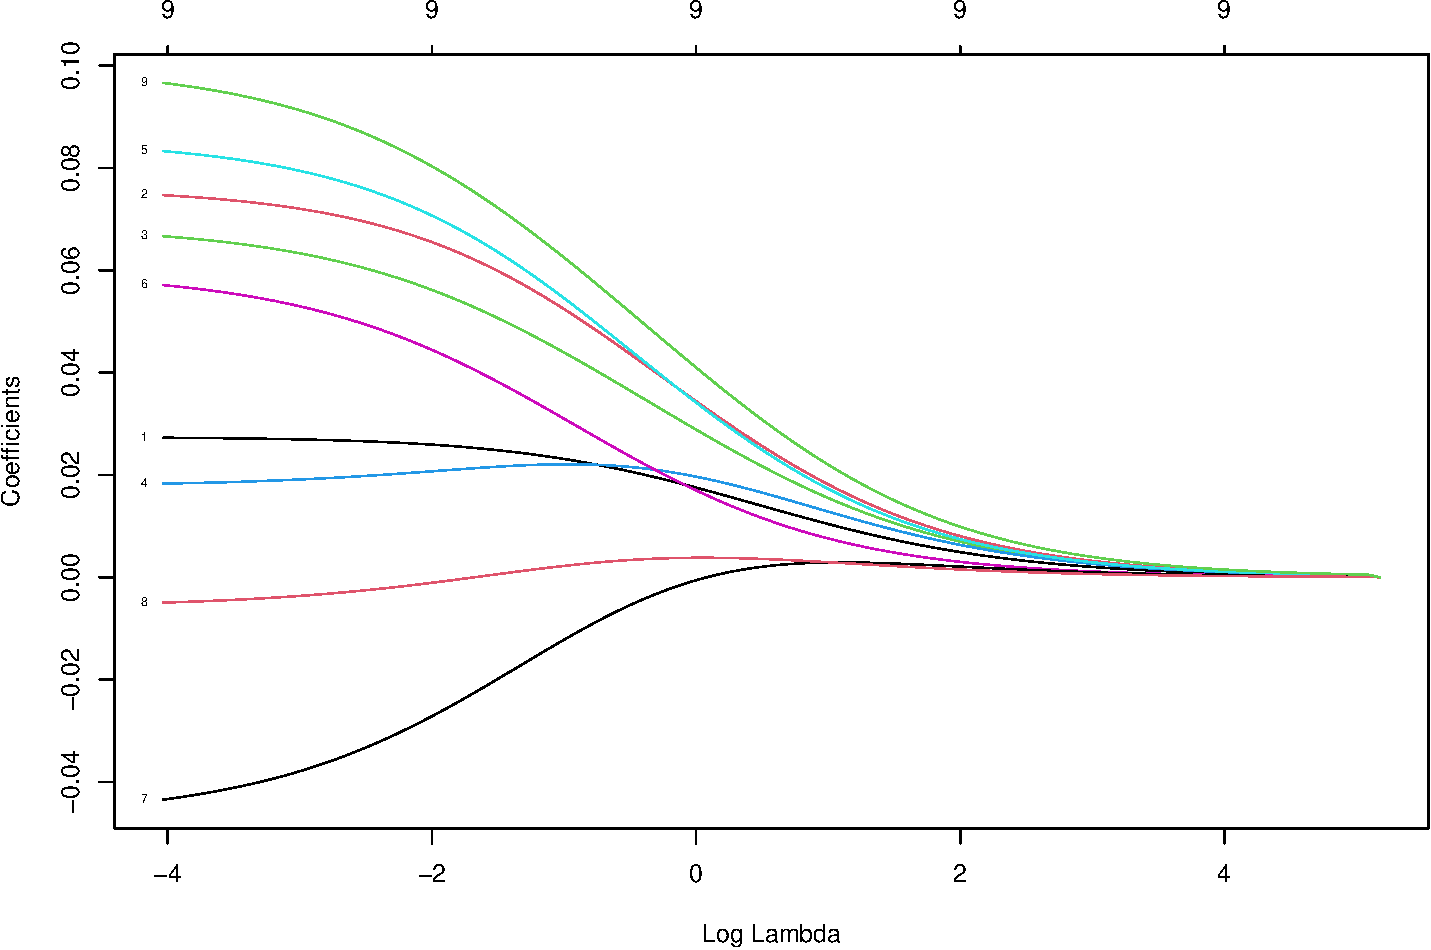
\includegraphics{L3_files/figure-beamer/unnamed-chunk-7-1.pdf}

\begin{Shaded}
\begin{Highlighting}[]
\NormalTok{cv.ridge=}\KeywordTok{cv.glmnet}\NormalTok{(}\DataTypeTok{x=}\NormalTok{xss,}\DataTypeTok{y=}\NormalTok{ys,}\DataTypeTok{alpha=}\DecValTok{0}\NormalTok{)}
\KeywordTok{print}\NormalTok{(}\KeywordTok{paste}\NormalTok{(}\StringTok{"The lamda giving the smallest CV error"}\NormalTok{,cv.ridge}\OperatorTok{$}\NormalTok{lambda.min))}
\end{Highlighting}
\end{Shaded}

\begin{verbatim}
## [1] "The lamda giving the smallest CV error 0.078625591076612"
\end{verbatim}

\begin{Shaded}
\begin{Highlighting}[]
\KeywordTok{print}\NormalTok{(}\KeywordTok{paste}\NormalTok{(}\StringTok{"The 1sd err method lambda"}\NormalTok{,cv.ridge}\OperatorTok{$}\NormalTok{lambda}\FloatTok{.1}\NormalTok{se))}
\end{Highlighting}
\end{Shaded}

\begin{verbatim}
## [1] "The 1sd err method lambda 0.668123660345539"
\end{verbatim}

\begin{Shaded}
\begin{Highlighting}[]
\KeywordTok{plot}\NormalTok{(cv.ridge)}
\end{Highlighting}
\end{Shaded}

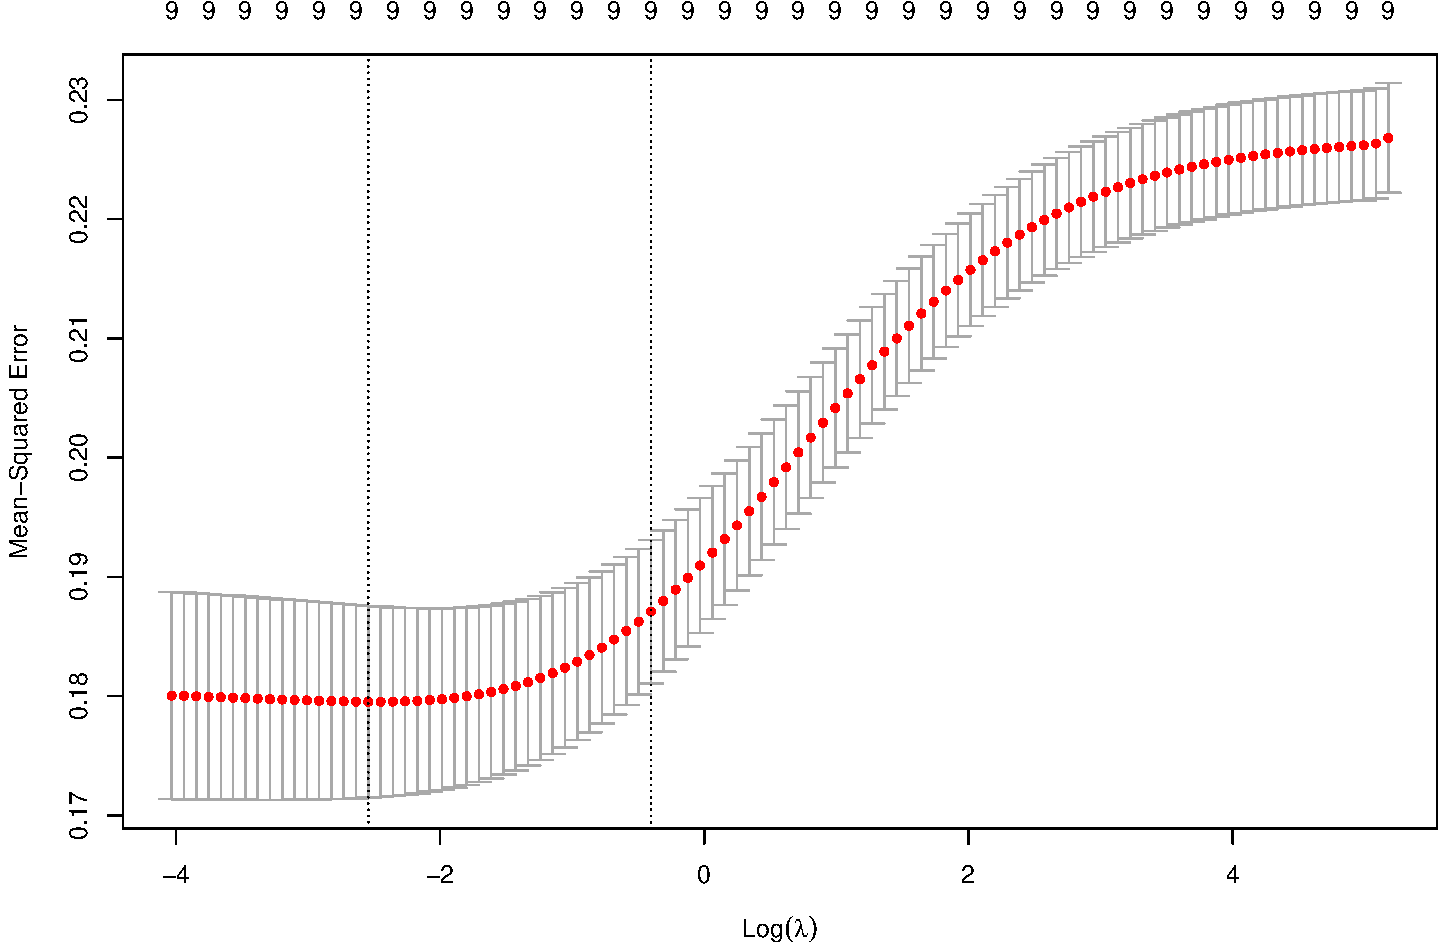
\includegraphics{L3_files/figure-beamer/unnamed-chunk-7-2.pdf}

\begin{Shaded}
\begin{Highlighting}[]
\CommentTok{# use 1sd error rule default}
\KeywordTok{plot}\NormalTok{(ridgefit,}\DataTypeTok{xvar=}\StringTok{"lambda"}\NormalTok{,}\DataTypeTok{label=}\OtherTok{TRUE}\NormalTok{);}
\KeywordTok{abline}\NormalTok{(}\DataTypeTok{v=}\KeywordTok{log}\NormalTok{(cv.ridge}\OperatorTok{$}\NormalTok{lambda}\FloatTok{.1}\NormalTok{se));}
\end{Highlighting}
\end{Shaded}

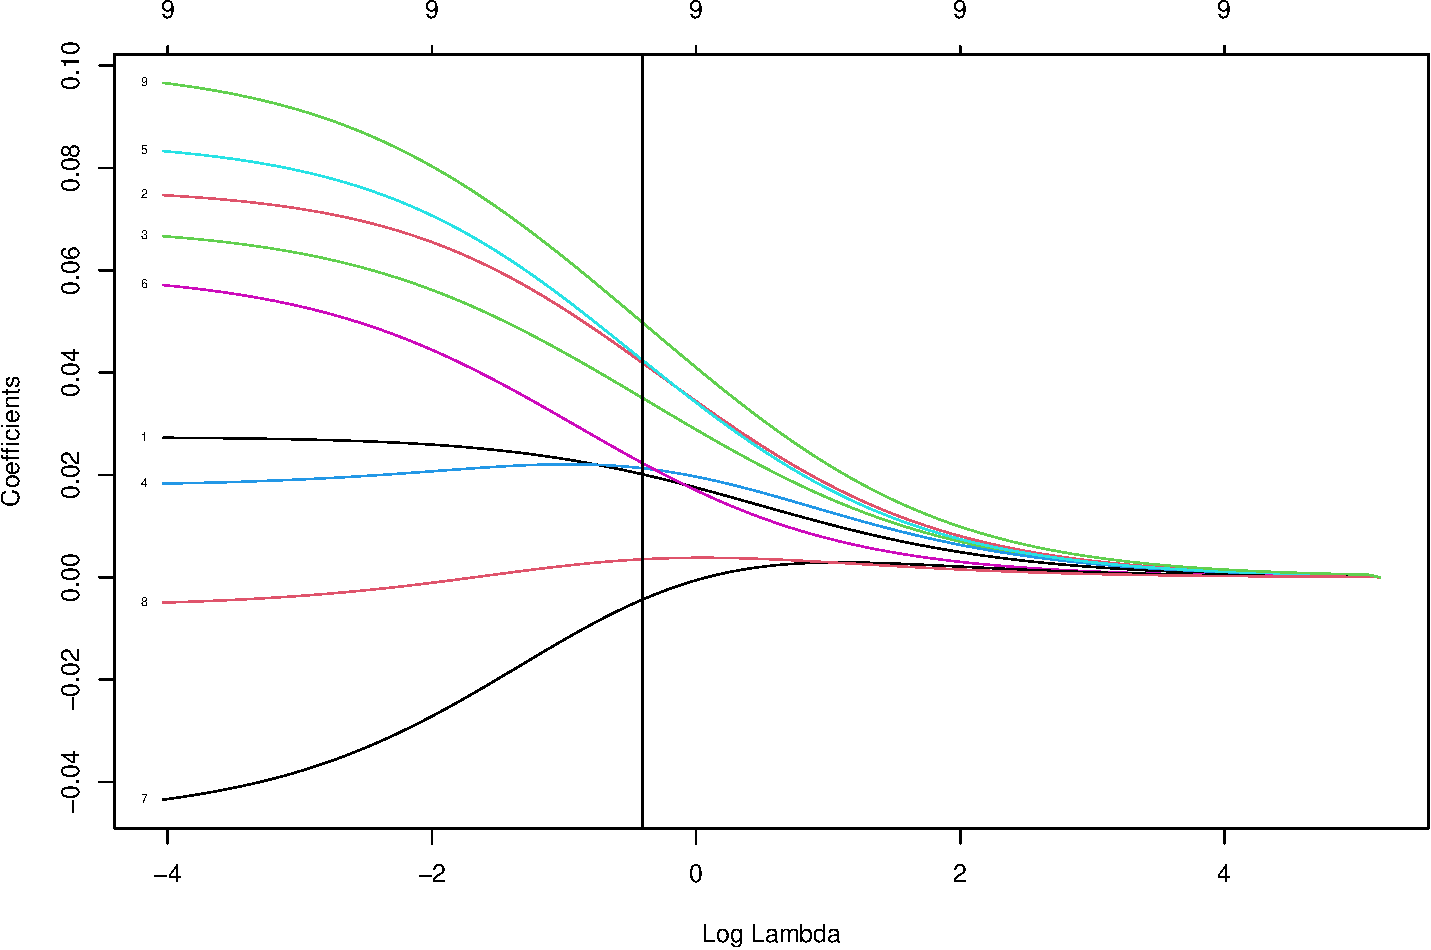
\includegraphics{L3_files/figure-beamer/unnamed-chunk-7-3.pdf}

\begin{Shaded}
\begin{Highlighting}[]
\KeywordTok{print}\NormalTok{(}\KeywordTok{cbind}\NormalTok{(}\KeywordTok{coef}\NormalTok{(ridgefit,}\DataTypeTok{s=}\NormalTok{cv.ridge}\OperatorTok{$}\NormalTok{lambda}\FloatTok{.1}\NormalTok{se),}\KeywordTok{coef}\NormalTok{(glm_heart)))}
\end{Highlighting}
\end{Shaded}

\begin{verbatim}
## 10 x 2 sparse Matrix of class "dgCMatrix"
##                           1             
## (Intercept)     0.346320346 -0.878545196
## sbp             0.020122344  0.133308398
## tobacco         0.041880099  0.364577926
## ldl             0.035011803  0.360180594
## adiposity       0.021312709  0.144616485
## famhistPresent  0.042403156  0.456537713
## typea           0.022293634  0.388725509
## obesity        -0.004329619 -0.265082072
## alcohol         0.003524355  0.002978424
## age             0.049743698  0.660695163
\end{verbatim}

\begin{Shaded}
\begin{Highlighting}[]
\CommentTok{# now possible to compare since the glm was also on standardized variables}
\end{Highlighting}
\end{Shaded}

\end{block}

\end{frame}

\begin{frame}[fragile]

\begin{block}{Lasso logistic regression}

Numbering in plots is order of covariates, so:

\begin{Shaded}
\begin{Highlighting}[]
\KeywordTok{cbind}\NormalTok{(}\DecValTok{1}\OperatorTok{:}\DecValTok{9}\NormalTok{,}\KeywordTok{colnames}\NormalTok{(xss))}
\end{Highlighting}
\end{Shaded}

\begin{verbatim}
##       [,1] [,2]            
##  [1,] "1"  "sbp"           
##  [2,] "2"  "tobacco"       
##  [3,] "3"  "ldl"           
##  [4,] "4"  "adiposity"     
##  [5,] "5"  "famhistPresent"
##  [6,] "6"  "typea"         
##  [7,] "7"  "obesity"       
##  [8,] "8"  "alcohol"       
##  [9,] "9"  "age"
\end{verbatim}

\begin{Shaded}
\begin{Highlighting}[]
\NormalTok{lassofit=}\KeywordTok{glmnet}\NormalTok{(}\DataTypeTok{x=}\NormalTok{xss,}\DataTypeTok{y=}\NormalTok{ys,}\DataTypeTok{alpha=}\DecValTok{1}\NormalTok{,}\DataTypeTok{standardize=}\OtherTok{FALSE}\NormalTok{) }\CommentTok{# already standardized}
\KeywordTok{plot}\NormalTok{(lassofit,}\DataTypeTok{xvar=}\StringTok{"lambda"}\NormalTok{,}\DataTypeTok{label=}\OtherTok{TRUE}\NormalTok{)}
\end{Highlighting}
\end{Shaded}

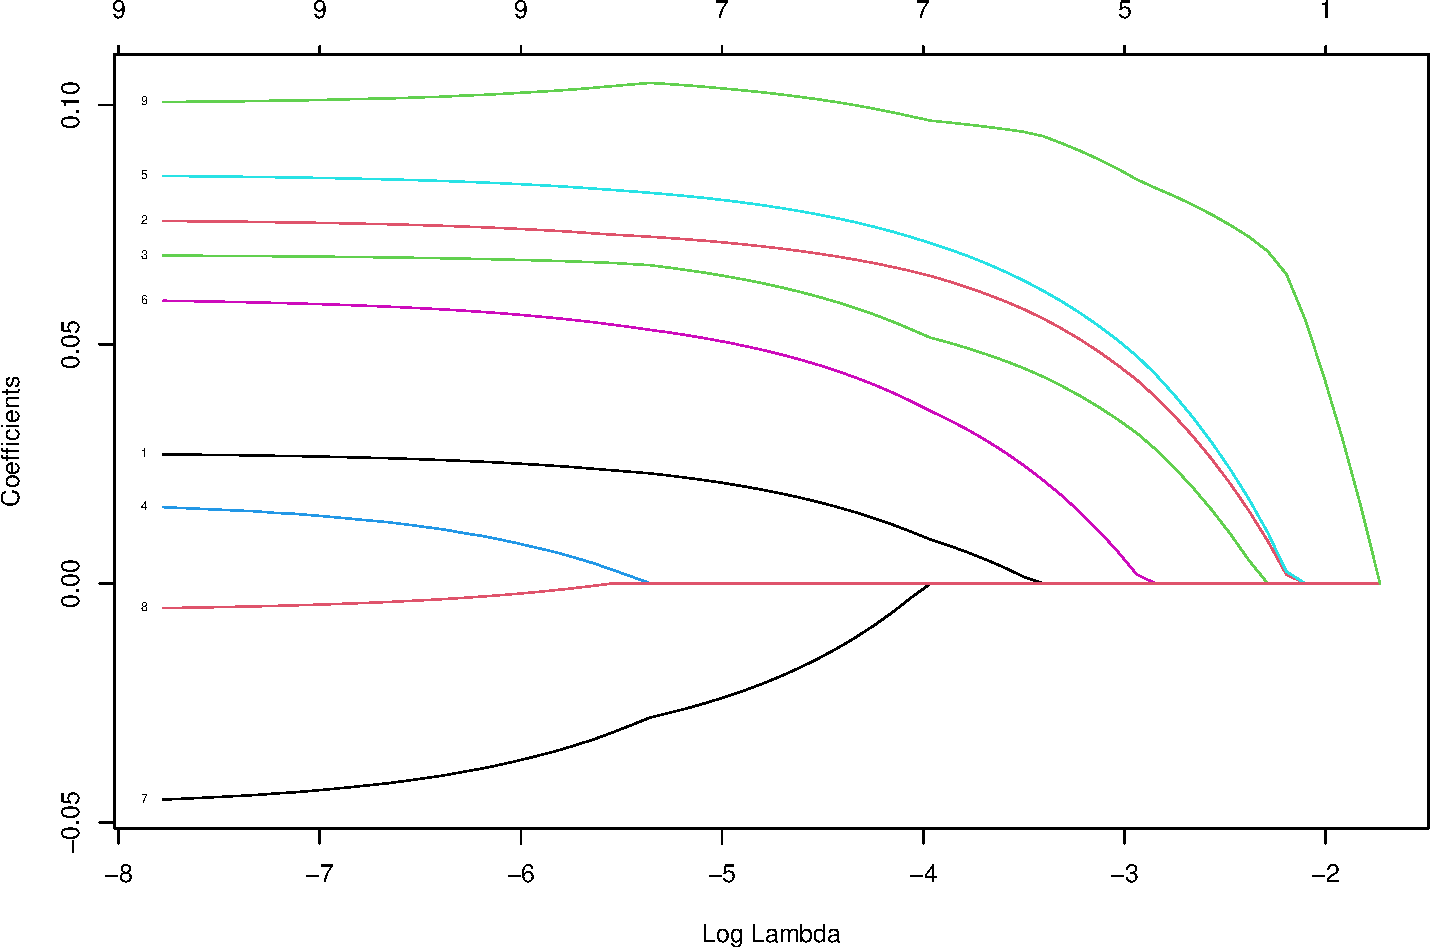
\includegraphics{L3_files/figure-beamer/unnamed-chunk-8-1.pdf}

\begin{Shaded}
\begin{Highlighting}[]
\NormalTok{cv.lasso=}\KeywordTok{cv.glmnet}\NormalTok{(}\DataTypeTok{x=}\NormalTok{xss,}\DataTypeTok{y=}\NormalTok{ys,}\DataTypeTok{alpha=}\DecValTok{1}\NormalTok{)}
\KeywordTok{print}\NormalTok{(}\KeywordTok{paste}\NormalTok{(}\StringTok{"The lamda giving the smallest CV error"}\NormalTok{,cv.lasso}\OperatorTok{$}\NormalTok{lambda.min))}
\end{Highlighting}
\end{Shaded}

\begin{verbatim}
## [1] "The lamda giving the smallest CV error 0.00904003229581495"
\end{verbatim}

\begin{Shaded}
\begin{Highlighting}[]
\KeywordTok{print}\NormalTok{(}\KeywordTok{paste}\NormalTok{(}\StringTok{"The 1sd err method lambda"}\NormalTok{,cv.lasso}\OperatorTok{$}\NormalTok{lambda}\FloatTok{.1}\NormalTok{se))}
\end{Highlighting}
\end{Shaded}

\begin{verbatim}
## [1] "The 1sd err method lambda 0.0482439333279146"
\end{verbatim}

\begin{Shaded}
\begin{Highlighting}[]
\KeywordTok{plot}\NormalTok{(cv.lasso)}
\end{Highlighting}
\end{Shaded}

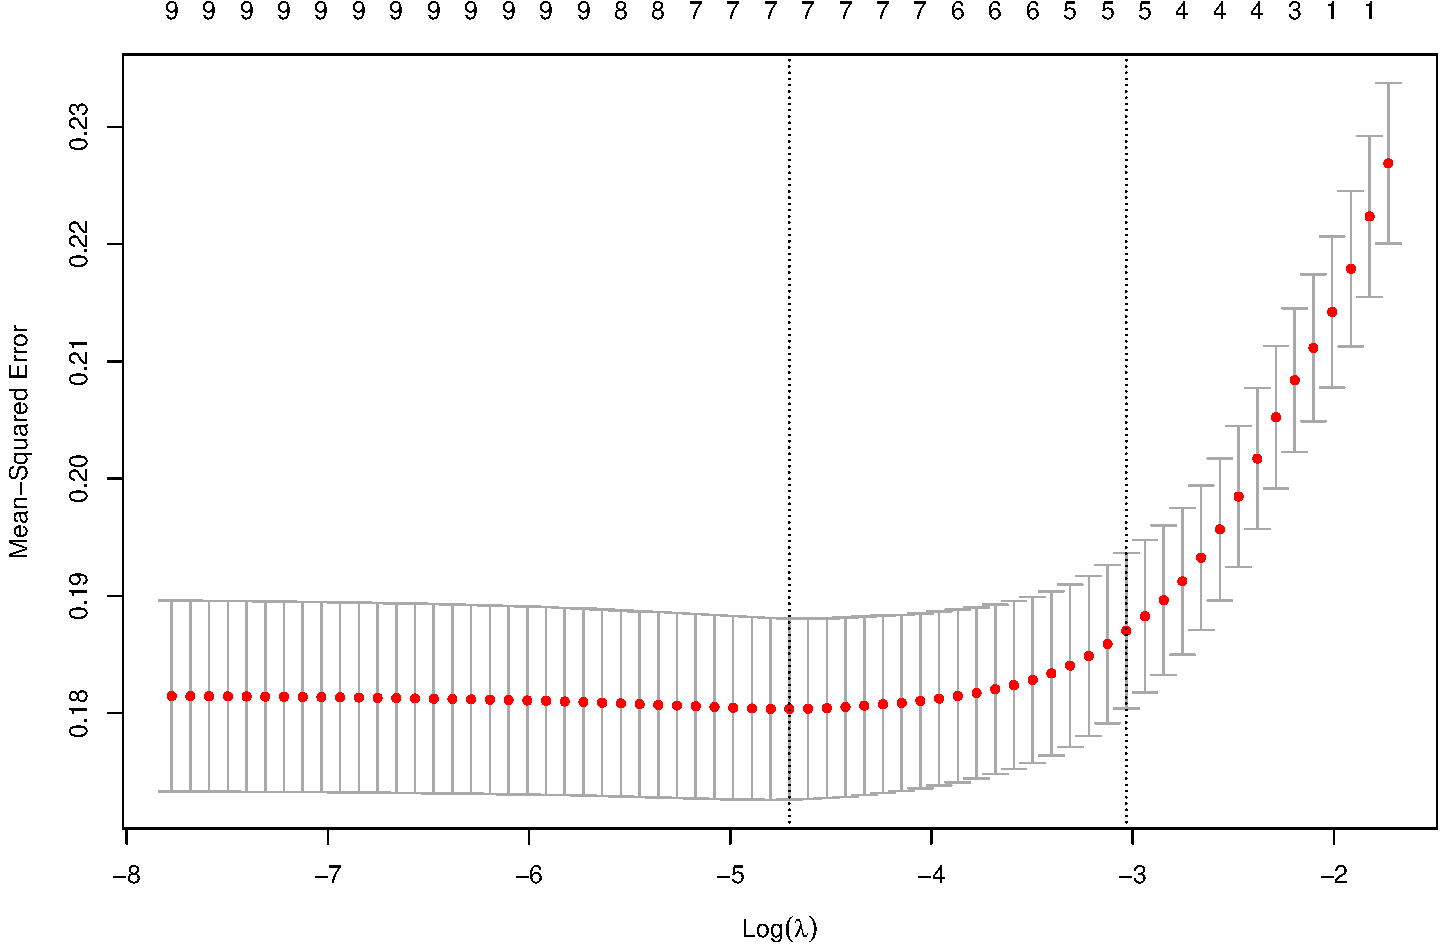
\includegraphics{L3_files/figure-beamer/unnamed-chunk-8-2.pdf}

\begin{Shaded}
\begin{Highlighting}[]
\CommentTok{# use 1sd error rule default}
\KeywordTok{plot}\NormalTok{(lassofit,}\DataTypeTok{xvar=}\StringTok{"lambda"}\NormalTok{,}\DataTypeTok{label=}\OtherTok{TRUE}\NormalTok{);}
\KeywordTok{abline}\NormalTok{(}\DataTypeTok{v=}\KeywordTok{log}\NormalTok{(cv.lasso}\OperatorTok{$}\NormalTok{lambda}\FloatTok{.1}\NormalTok{se));}
\end{Highlighting}
\end{Shaded}

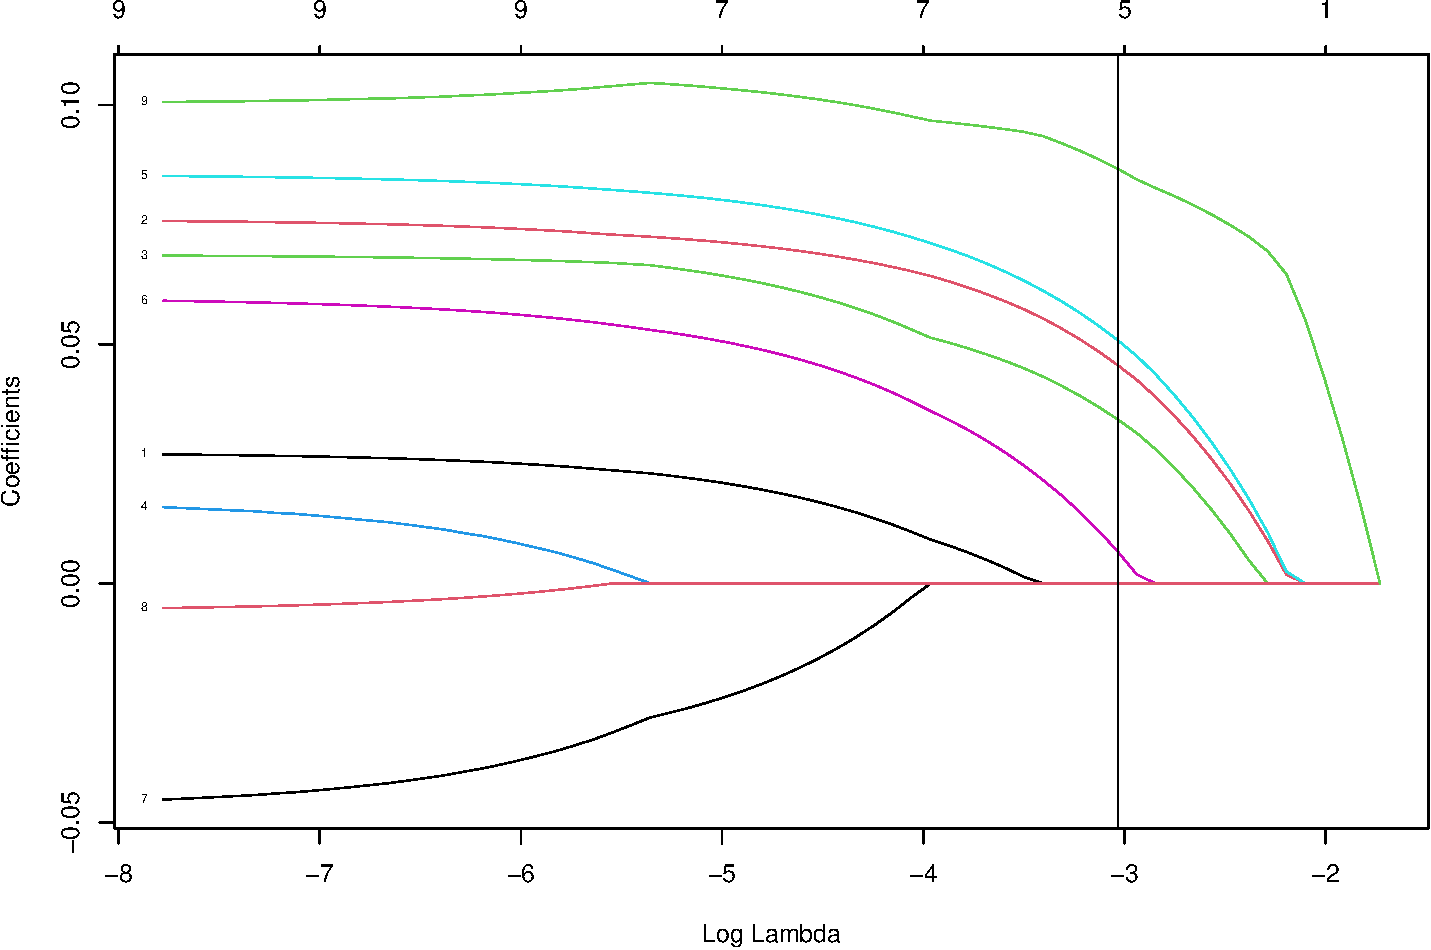
\includegraphics{L3_files/figure-beamer/unnamed-chunk-8-3.pdf}

\begin{Shaded}
\begin{Highlighting}[]
\NormalTok{resmat=}\KeywordTok{cbind}\NormalTok{(}\KeywordTok{coef}\NormalTok{(lassofit,}\DataTypeTok{s=}\NormalTok{cv.lasso}\OperatorTok{$}\NormalTok{lambda}\FloatTok{.1}\NormalTok{se),}\KeywordTok{coef}\NormalTok{(ridgefit,}\DataTypeTok{s=}\NormalTok{cv.ridge}\OperatorTok{$}\NormalTok{lambda}\FloatTok{.1}\NormalTok{se),}\KeywordTok{coef}\NormalTok{(glm_heart))}
\KeywordTok{colnames}\NormalTok{(resmat)=}\KeywordTok{c}\NormalTok{(}\StringTok{"lasso logistic"}\NormalTok{,}\StringTok{"ridge logistic"}\NormalTok{,}\StringTok{"logistic"}\NormalTok{)}
\KeywordTok{print}\NormalTok{(resmat)}
\end{Highlighting}
\end{Shaded}

\begin{verbatim}
## 10 x 3 sparse Matrix of class "dgCMatrix"
##                lasso logistic ridge logistic     logistic
## (Intercept)       0.346320346    0.346320346 -0.878545196
## sbp               .              0.020122344  0.133308398
## tobacco           0.045556402    0.041880099  0.364577926
## ldl               0.034213019    0.035011803  0.360180594
## adiposity         .              0.021312709  0.144616485
## famhistPresent    0.050771463    0.042403156  0.456537713
## typea             0.006558737    0.022293634  0.388725509
## obesity           .             -0.004329619 -0.265082072
## alcohol           .              0.003524355  0.002978424
## age               0.086624979    0.049743698  0.660695163
\end{verbatim}

\end{block}

\end{frame}

\begin{frame}[fragile]{Computational details for the glmnet
implementation}
\protect\hypertarget{computational-details-for-the-glmnet-implementation}{}

(HTW 3.7)

\texttt{glmnet} is the implementation in R of the elastic net from
HTW-book, and the package is maintained by Trevor Hastie.

The package fits generalized linear models using penalized maximum
likelihood of elastic net type (lasso and ridge are special cases).

The logistic lasso is fitted using a quadratic approximation for the
negative log-likelihood in a ``proximal-Newton iterative approach''.

\begin{block}{Software links}

\begin{itemize}
\tightlist
\item
  \href{https://cran.r-project.org/web/packages/glmnet/index.html}{R
  glmnet on CRAN} with
  \href{http://www.stanford.edu/~hastie/glmnet}{resources}.

  \begin{itemize}
  \tightlist
  \item
    \href{https://glmnet.stanford.edu/articles/glmnet.html}{Getting
    started}
  \item
    \href{https://glmnet.stanford.edu/articles/glmnetFamily.html}{GLM
    with glmnet}
  \end{itemize}
\end{itemize}

For Python there are different options.

\begin{itemize}
\tightlist
\item
  \href{https://web.stanford.edu/~hastie/glmnet_python/}{Python glmnet}
  is recommended by Hastie et al.
\item
  \href{https://scikit-learn.org/stable/modules/linear_model.html\#ridge-regression-and-classification}{scikit-learn}
  (seems to mostly be for regression? is there lasso for classification
  here?)
\end{itemize}

\end{block}

\end{frame}

\begin{frame}[fragile]

\begin{block}{glmnet inputs}

\begin{Shaded}
\begin{Highlighting}[]
\KeywordTok{glmnet}\NormalTok{(x, y, }
 \DataTypeTok{family =} \KeywordTok{c}\NormalTok{(}\StringTok{"gaussian"}\NormalTok{, }\StringTok{"binomial"}\NormalTok{, }\StringTok{"poisson"}\NormalTok{, }\StringTok{"multinomial"}\NormalTok{,}\StringTok{"cox"}\NormalTok{, }\StringTok{"mgaussian"}\NormalTok{),}
 \DataTypeTok{weights =} \OtherTok{NULL}\NormalTok{, }\DataTypeTok{offset =} \OtherTok{NULL}\NormalTok{, }\DataTypeTok{alpha =} \DecValTok{1}\NormalTok{, }\DataTypeTok{nlambda =} \DecValTok{100}\NormalTok{, }
 \DataTypeTok{lambda.min.ratio =} \KeywordTok{ifelse}\NormalTok{(nobs }\OperatorTok{<}\StringTok{ }\NormalTok{nvars, }\FloatTok{0.01}\NormalTok{, }\FloatTok{1e-04}\NormalTok{),}
 \DataTypeTok{lambda =} \OtherTok{NULL}\NormalTok{, }\DataTypeTok{standardize =} \OtherTok{TRUE}\NormalTok{, }\DataTypeTok{intercept =} \OtherTok{TRUE}\NormalTok{,}
 \DataTypeTok{thresh =} \FloatTok{1e-07}\NormalTok{, }\DataTypeTok{dfmax =}\NormalTok{ nvars }\OperatorTok{+}\StringTok{ }\DecValTok{1}\NormalTok{, }
 \DataTypeTok{pmax =} \KeywordTok{min}\NormalTok{(dfmax }\OperatorTok{*}\StringTok{ }\DecValTok{2} \OperatorTok{+}\StringTok{ }\DecValTok{20}\NormalTok{, nvars), }
 \DataTypeTok{exclude =} \OtherTok{NULL}\NormalTok{, }\DataTypeTok{penalty.factor =} \KeywordTok{rep}\NormalTok{(}\DecValTok{1}\NormalTok{, nvars),}
 \DataTypeTok{lower.limits =} \OperatorTok{-}\OtherTok{Inf}\NormalTok{, }\DataTypeTok{upper.limits =} \OtherTok{Inf}\NormalTok{, }\DataTypeTok{maxit =} \FloatTok{1e+05}\NormalTok{,}
 \DataTypeTok{type.gaussian =} \KeywordTok{ifelse}\NormalTok{(nvars }\OperatorTok{<}\StringTok{ }\DecValTok{500}\NormalTok{, }\StringTok{"covariance"}\NormalTok{, }\StringTok{"naive"}\NormalTok{),}
 \DataTypeTok{type.logistic =} \KeywordTok{c}\NormalTok{(}\StringTok{"Newton"}\NormalTok{, }\StringTok{"modified.Newton"}\NormalTok{),}
 \DataTypeTok{standardize.response =} \OtherTok{FALSE}\NormalTok{, }
 \DataTypeTok{type.multinomial =} \KeywordTok{c}\NormalTok{(}\StringTok{"ungrouped"}\NormalTok{,}\StringTok{"grouped"}\NormalTok{), }
 \DataTypeTok{relax =} \OtherTok{FALSE}\NormalTok{, }\DataTypeTok{trace.it =} \DecValTok{0}\NormalTok{, ...)}
\end{Highlighting}
\end{Shaded}

\end{block}

\end{frame}

\begin{frame}[fragile]

\begin{block}{cv.glmnet inputs}

\begin{Shaded}
\begin{Highlighting}[]
\KeywordTok{cv.glmnet}\NormalTok{(x, y, }\DataTypeTok{weights =} \OtherTok{NULL}\NormalTok{, }\DataTypeTok{offset =} \OtherTok{NULL}\NormalTok{, }\DataTypeTok{lambda =} \OtherTok{NULL}\NormalTok{,}
  \DataTypeTok{type.measure =} \KeywordTok{c}\NormalTok{(}\StringTok{"default"}\NormalTok{, }\StringTok{"mse"}\NormalTok{, }\StringTok{"deviance"}\NormalTok{, }\StringTok{"class"}\NormalTok{, }\StringTok{"auc"}\NormalTok{, }\StringTok{"mae"}\NormalTok{,}\StringTok{"C"}\NormalTok{),}
  \DataTypeTok{nfolds =} \DecValTok{10}\NormalTok{, }\DataTypeTok{foldid =} \OtherTok{NULL}\NormalTok{, }
  \DataTypeTok{alignment =} \KeywordTok{c}\NormalTok{(}\StringTok{"lambda"}\NormalTok{, }\StringTok{"fraction"}\NormalTok{), }\DataTypeTok{grouped =} \OtherTok{TRUE}\NormalTok{, }
  \DataTypeTok{keep =} \OtherTok{FALSE}\NormalTok{, }\DataTypeTok{parallel =} \OtherTok{FALSE}\NormalTok{,}
  \DataTypeTok{gamma =} \KeywordTok{c}\NormalTok{(}\DecValTok{0}\NormalTok{, }\FloatTok{0.25}\NormalTok{, }\FloatTok{0.5}\NormalTok{, }\FloatTok{0.75}\NormalTok{, }\DecValTok{1}\NormalTok{), }\DataTypeTok{relax =} \OtherTok{FALSE}\NormalTok{, }\DataTypeTok{trace.it =} \DecValTok{0}\NormalTok{, ...)}
\end{Highlighting}
\end{Shaded}

type.measure defaults to deviance (accoring to help(cv.glmnet)). The
last is for Cox models.

\end{block}

\end{frame}

\begin{frame}[fragile]

\begin{block}{Family}

we have only covered \texttt{gaussian} (the default) and
\texttt{binomial}.

Each family has implemented the deviance measure. Poisson regression and
Cox proportional hazard (survival analysis) is also implemented in
glmnet.

\end{block}

\end{frame}

\begin{frame}

\begin{block}{Penalties}

The elastic net is implemented, with three possible adjustment
parameters.

\[ \text{minimize}_{\beta_0,\beta} \{ -\frac{1}{N} l(y;\beta_0,\beta)+\lambda \sum_{j=1}^p
\gamma_j ((1-\alpha)\beta_j^2+\alpha \lvert \beta_j \rvert)\}\]

\begin{itemize}
\tightlist
\item
  \(\lambda\): the penalty, default a grid of 100 values is chosen, to
  cover the lasso path on the log scale.
\item
  \(\alpha\): elastic net parameter \(\in [0,1]\). This is usually
  manually selected by a grid search over 3-5 values. Default is
  \(\alpha=1\) (lasso), and with \(\alpha=0\) we get ridge.
\item
  \(\gamma_j\): penalty modifier for each covariate to be able to always
  include (\(\gamma_j==0\)), or exclude (\(\gamma_j=\text{Inf}\)), or
  give individual penalty modifications. Default \(\lambda_j=1\).
\end{itemize}

\end{block}

\end{frame}

\begin{frame}

For the \(\lambda\) penalty the maximal value is for

\begin{itemize}
\tightlist
\item
  linear regression:
  \(\lambda_{\text max}=\text{max}_j \lvert \hat{\beta}_{LS,j} \rvert\)
  (standardized coefficients) or, should there also be a factor 1/N?
\item
  logistic regression:
  \(\lambda_{\text max}=\text{max}_{j}\lvert {\bf x}_j ^T ({\bf y}-\bar{p}) \rvert\)
  where \(\bar p\) is the mean case rate.
\end{itemize}

\begin{block}{Additional modifications}

\begin{itemize}
\tightlist
\item
  Coefficient bounds can be set (possible since coordinate descent is
  used)
\item
  Some coefficients can be excluded from the penalization (than thus
  forced in).
\item
  Offset can be added (popular if rate models for Poisson is used)
\item
  For binary and multinomial data factors or matrices can be input.
\item
  Sparse matrices with covariates can be supplied.
\end{itemize}

\end{block}

\end{frame}

\begin{frame}

\begin{block}{Lasso variants}

Elastic net is already in glmnet (alpha-parameter).

Other lasso variants have their own R packages:

\begin{itemize}
\item
  The group lasso
  \url{https://cran.r-project.org/web/packages/grplasso/grplasso.pdf}
\item
  The fused lasso
  \url{https://cran.r-project.org/web/packages/genlasso/genlasso.pdf}
\item
  Bayesian lasso blasso function for normal data in package monomvn
  \url{https://rdrr.io/cran/monomvn/man/monomvn-package.html}
\item
  Elastic net for ordinal data:
  \url{https://cran.r-project.org/web/packages/ordinalNet/ordinalNet.pdf}
\end{itemize}

\end{block}

\end{frame}

\begin{frame}[fragile]{Exercises}
\protect\hypertarget{exercises}{}

This week the best way to spend the time is to work on the Data Analysis
Project 1.

But, also good to study the R-code for the South African heart disease
example, and make some changes.

\textbf{Smart:} save this file as an .Rmd file and then run
\texttt{purl(file.Rmd)} to produce a file with only the R-commands. (At
the html-version you choose Code-Download Rmd on the top of the file).

\begin{itemize}
\tightlist
\item
  Change the CV criterion to auc and to class. Are there changes?
\end{itemize}

\end{frame}

\begin{frame}{References}
\protect\hypertarget{references}{}

\begin{itemize}
\tightlist
\item
  Robert Tibshirani Regression Shrinkage and Selection via the Lasso,
  Journal of the Royal Statistical Society. Series B (Methodological)
  Vol. 58, No.~1 (1996), pp.~267-288 (22 pages)
\item
  \href{https://arxiv.org/pdf/1509.09169.pdf}{Lecture notes on ridge
  regression: Welle N. van Wieringen}
\end{itemize}

\end{frame}

\end{document}
